\documentclass{article}

\usepackage[margin=.75in]{geometry}
\usepackage{listings}
\usepackage{amsmath}
\usepackage[shortlabels]{enumitem}
\usepackage{tikz}
\usetikzlibrary{arrows, %
                shapes, positioning}

\lstset{
    basicstyle=\ttfamily,
    mathescape
}

\author{Damien Prieur}
\title{Homework 2 \\ CS 458}
\date{}

\begin{document}

\maketitle

\section*{Problem 1}
An ordered stack is a data structure that stores a sequence of items and supports the following operations.
\begin{itemize}
\item $Push'(x)$ removes all items smaller than x from the beginning of the sequence and then adds $x$ to the beginning of the sequence.
\item $Pop$ deletes and returns the first item in the sequence.
\end{itemize}
\indent Prove that if we start with and empty data structure, the amortized cost of each $Push'$ and $Pop$ operation is $O(1)$.
\newline
\newline
\indent Approaching this using the Potential Method.
Let $\phi (D_i)$ be the number of elements in the stack.
For each operation we look at how $\phi(D)$ changes.
\newline
\newline
\begin{tabular}{r l}
                & The real cost $c_i$ is $1$ as we are just removing an item from the stack. \\
    $Pop$:      & The potential difference is $\phi(D_i)-\phi(D_{i-1}) = -1$ since we are removing one item from the stack. \\
                & Therefore the amortized cost is $\hat{c}_i = c_i + \phi(D_i)-\phi(D_{i-1}) = 1 - 1 = 0$ which is constant. \\
                \\
                & The real cost $c_i$ is $1 + k$ where $k = $ the number of elements that are smaller than $x$ \\
    $Push'(x)$: & The potential difference is $(\phi(D_i)-\phi(D_{i-1}) = (\phi(D_{i-1}) - k + 1) - \phi(D_{i-1}) = -k + 1 $ \\
                & Therefore the amortized cost is $\hat{c}_i = c_i + \phi(D_i)-\phi(D_{i-1}) = 1 + k - k + 1 = 2$ which is constant \\
\end{tabular}
\newline
\newline
Since we are starting with an empty stack $\phi(D_0) = 0$.
We can also show that $\phi(D_i) \geq 0 \text{ for all } i$ as the stack cannot have ``negative items" inside of it.
The $Push'(x)$ operation is the only thing that could drop the potential below $0$, but the number of items it can remove is capped at the number of items in the stack.
\\
Therefore the ordered stack's operations $Pop$ and $Push'(x)$ are $O(1)$.

\newpage
\section*{Problem 2}
You're in charge of food rationing, or as the locals call it, \emph{the dining halls}.
Every person is assigned to a dining hall.
These assignments are based on where the people live - the municipal government has decreed that no person should have to travel more than a quarter mile from their house to get to a dining hall.
After making this promise, the government realized that implementing this plan might be a bit tricky; as you may know dining halls aren't great places when they're over-congested.
Your job is to figure out if there's a way to feed everyone without overtaxing any one dining hall.
\\
\indent Formally, you're given a list of all $n$ people and a list of the $m$ dining halls.
Each person $i$ is within a quarter mile of some set $S_i$ of dining halls, and must be assigned to some dining hall in $S_i$.
Each dining hall $j$ has a capacity $C_j$, which is an upper limit on the number of people it can feed.
Your job is to assign people to dining halls in a way that feeds all people and doesn't overtax any dining hall.
Give an algorithm that computes such an assignment, or outputs that no such assignment exists.
Your algorithm should return in time polynomial in $n$ and $m$. Analyze your algorithm's runtime and prove that it is correct.
\\
\indent You may use any algorithm we studied during lecture for max flow as a black box.
Mention which you are using in your runtime analysis.
\newline
\newline
\indent We need to reduce this problem to a flow problem.
To do this we attach all the students to a super source that has a capacity of $1$ to represent the fact that a student is assigned to one and only one dining hall.
Then for each $i$ we attach an edge from $i$ to each dining hall in $S_i$ with a capacity of 1, this capacity doesn't actually matter since the students are restricted from the super source capacity of one to each student.
Then we attach each dining hall $j$ to a super sink with capacity $C_j$ so that they can't be assigned more students than their capacity.
With this setup we run a max flow algorithm and see if $|f| = n$ it can't be larger than that since the only way out of the source node is through each student.
If all students are being used then we get a max flow of $|f| = n$, but if $|f| < n$ then we don't have a solution.
The dining halls cannot be matched to students with the distance and capacity constraints.
If there is a solution the assignment of students to dining halls will be exactly the flows between the students $i$ and the dining halls $j$.
\newline
\newline
\begin{figure}[!h]
\centering
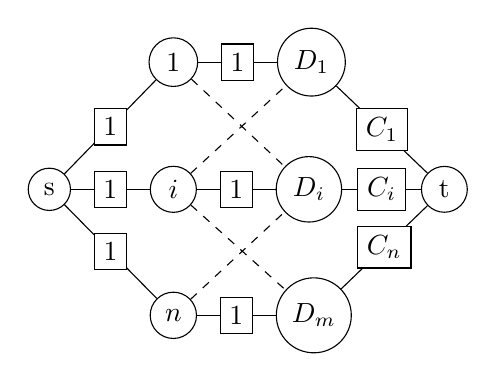
\begin{tikzpicture}
    \tikzset{LabelStyle/.style = {draw, fill=white}}
    \tikzset{VertexStyle/.style = {circle, draw=black}}
    \node[VertexStyle](s){s};
    \node[VertexStyle, right=of s](Si){$i$};
    \node[VertexStyle, above=of Si](S1){$1$};
    \node[VertexStyle, below=of Si](Sn){$n$};
    \node[VertexStyle, right=of S1](D1){$D_{1}$};
    \node[VertexStyle, right=of Si](Di){$D_{i}$};
    \node[VertexStyle, right=of Sn](Dm){$D_{m}$};
    \node[VertexStyle, right=of Di](t){t};
    \draw(s) to node[LabelStyle]{1} (Si);
    \draw(s) to node[LabelStyle]{1} (S1);
    \draw(s) to node[LabelStyle]{1} (Sn);
    \draw(S1) to node[LabelStyle]{1} (D1);
    \draw(Si) to node[LabelStyle]{1} (Di);
    \draw(Sn) to node[LabelStyle]{1} (Dm);

    \draw[dashed](S1) to node{} (Di);
    \draw[dashed](Si) to node{} (D1);
    \draw[dashed](Si) to node{} (Dm);
    \draw[dashed](Sn) to node{} (Di);

    \draw(D1) to node[LabelStyle]{$C_1$} (t);
    \draw(Di) to node[LabelStyle]{$C_i$} (t);
    \draw(Dm) to node[LabelStyle]{$C_n$} (t);
\end{tikzpicture}
\end{figure}
\newline
\newline
\indent The runtime of this algorithm would be the initial cost of creating the graph then the cost of computing the max flow.
The cost of creating the graph will be equal to the number of nodes and edges.
The number of nodes is equal to $2 + n + m$ which comes from the super source and super sink nodes, and a node for each student and building.
The number of edges will depend on $S_i$ as well, but it can be upper bounded by $m$ as a student can't be assigned to more than the number of dining halls.
This makes the number of edges $= n + m + \sum_{i}S_i$ since the source is connected to each student once, the sink is connected to each dining hall, and the last term is summing all dining halls in range for each student.
With the upper bound on $S_i$ we can put a worse case on the number of edges as $n + m + \sum_{i}m = n + m + nm$.
Therefore the cost to create the initial graph will be equal to the sum of creating the nodes and edges as those can each be made in constant time by using an adjacency matrix.
$$ Cost = 2 + n + m + n + m + nm = nm + 2(1 + n + m) \in O(nm) $$
The cost of finding the max flow using Ford Fulkerson is $O(VE^2)$ in terms of $n$ and $m$ is $O((2+n+m)\cdot(n + m + nm)^2)$.
We can rewrite this.

$$ O((2+n+m)\cdot(n + m + nm)^2) \in O((n+m)\cdot(nm)^2) = O(n^3m^2 + n^2m^3)$$


\newpage
\section*{Problem 3}
One intuitive story for the max flow problem is that the input graph $G = (V,E)$ is a rail network, the capacities are shipping capacities along rail lines, and the algorithm designer interested in maximizing the volume of shipments from some source city $s$ to the sink city $t$.
\\
\indent You're interested in ruining this particular algorithm designer's plans.
Specifically, we're given a rail network $G = (V,E)$ with \emph{unit capacities}, a source $s$, and a sink $t$.
We have enough explosives to destroy $d$ rails.
Our goal is to reduce the volume of shipping between $s$ and sink $t$ (computed via max flow) by as much as possible.
The question is: which ones should we destroy?
\\
\indent Give an efficient algorithm which takes $G$,$s$,$t$, and $d$ as inputs, and returns a set of rails $S \subseteq E$ which , when removed, reduces the total shipments from $s$ to $t$ by the maximum amount.
Prove correctness and runtime for your algorithm.
\newline
\newline
\indent Find the min cut and choose the edge with the used capacity (flow) and destroy that edge.
When you cut an edge you are guaranteed to drop the flow by the amount of the used capacity of the edge that is removed by the min-cut theorem.
The cut that you now have will also cut the new flow, and by the min-cut theorem it is the new min-cut of the flow graph without the edge that was removed.
Remove as many edges from the min cut as possible.
\newline
\newline
\indent To find the min-cut we can perform a node traversal on the residual graph after computing the max flow and mark edges that are saturated and go to a vertex that is not reachable.
These edges that are saturated towards an unreachable vertex in the residual graph belong to the min-cut.
\newline
\newline
\indent Using the Ford Fulkerson algorithm and BFS we can get a runtime of $O(VE^2 + V + E)$ for finding the min-cut.
Need to find $d$ edges to cut which requires a search on the edges along the cut which is bounded by the number of vertexes.
Therefore the runtime should be $O(VE^2 + V + E Vd) \in O(VE^2 + V^2)$ in the worse case as $d \leq V$.

\end{document}

